\documentclass[letterpaper]{article}%
\usepackage{fullpage}[10pt,onesided]%
\usepackage{titlesec}%
\usepackage{amsmath}%
\usepackage{amsfonts}%
\usepackage{enumerate}%
\usepackage{graphicx}%

\author{Brandon Reiss}
\date{Tuesday, May 8th, 2012}
\title{Robotics - Project}
\renewcommand{\thesection}{\Roman{section}}
\renewcommand{\thesubsection}{%
  \arabic{subsection} \setcounter{equation}{0}}

\begin{document}
\maketitle

\def\cpp{${\rm C}^{++}$}

\section*{Project Description}%

\subsection{Overview}
This document refers to experience working with the TurtleBot robotics package
from Willow Garage. The package consists of an iRobot Create drivetrain on top
of which is mounted a series of platforms up to approximately $0.5$m tall. The
package contains an ASUS 1215N netbook as an onboard computer. The
configuration used for this project supports an XBox Kinect sensor as well as a
robotic arm.

An extensive suite of software tools based on the Robot Operating System, or
ROS, are provided and maintained by Willow Garage. ROS is a publish/subscribe
architecture designed to flow data on-demand to system components expressed as
nodes. A topic is a single stream of data. Topics are addressed using paths
beginning with the Unix path separator character ``/''. For example, the Kinect
RGB image data are published by the {\tt openni\_camera} node on {\tt
/camera/rgb/image\_color}.

All code relevant to this project is stored on the nyu-robotics github
available at \linebreak
{\tt https://github.com/ylecun/nyu-robotics}. Special thanks to Prof. Lecun for
sharing literally hundreds of thousands of lines of code from Lush and other
projects as resources for this project.

\subsection{Scope}
The main focus of this project is to perform visual odometry as a basis for
building a coherent map of the environment surrounding the robot.
The work completed for this project falls into three major categories:
\begin{enumerate}
  \item RosLush -- a software library interfacing ROS with Lush
  \item TurtleBot driver -- a simple driving program
  \item Visual odometry -- odometry correction tools and procedures
\end{enumerate}

\section{RosLush}
A critical component of this project is the infrastructure required to control
the robot systems. Due to the abundance of packages existing in ROS, it was
chosen as the underlying method of interacting with the robot hardware.
However, since a great deal of resources for machine learning, computer vision,
and linear algebra were available in Lush, it was also very beneficial to have
a library to facilitate interaction between the two programming environments.

\subsection{Design}
RosLush is a \cpp{} library that supports a variety of essential topics and
message types used to control the TurtleBot. Its generic \cpp{} template-based
design allows clients to define new interfaces to ROS topics. By utilizing the
{\tt ros::spinonce()} API, the library allows Lush to retain control flow by
polling ROS topics for the newest data available. The {\tt turtlebot} Lush
package is built on RosLush.  A typical main loop using {\tt turtlebot}
performs the following steps:
\begin{enumerate}
  \item Start subscriptions to all desired topics \vspace{-10.0 pt}
    \begin{verbatim}
    (libload "local/turtlebot")
    (de main-loop ()
      (let ((tb (new turtlebot)))
        ;; Subscribe to topics.
        (==> tb start-sub-camera-rgb-image-color)
        (==> tb start-sub-camera-depth-points)
    \end{verbatim}
    \vspace{-20.0 pt}
  \item Enter a main loop \vspace{-10.0 pt}
    \begin{verbatim}
        ;; Loop forever.
        (while (t)
    \end{verbatim}
    \vspace{-20.0 pt}
  \item Wait for new data \vspace{-10.0 pt}
    \begin{verbatim}
          ;; Get new data from topics.
          (while (< (==> tb update-camera-rgb-image-color) 0))
          (while (< (==> tb update-camera-depth-points) 0))
    \end{verbatim}
    \vspace{-20.0 pt}
  \item Process data \vspace{-10.0 pt}
    \begin{verbatim}
          (make-robot-do-amazing-stuff
            :tb:camera-rgb-image-color :tb:camera-depth-points))))
    \end{verbatim}
    \vspace{-20.0 pt}
  \item Repeat $3 - 4$
\end{enumerate}
Each {\tt turtlebot} instance in Lush is a unique \cpp{} object that holds
state for the current message id grabbed from each topic as well as objects
that facilitate direct, no-copy access to the data received by ROS. The library
benefits from the fact that many parameters are configurable using ROS launch
scripts, and the {\tt openni\_camera} node performs automatic rectification of
the XYZRGB data.

For more documentation, see {\tt lush/local/ros/roslush.h} from the
nyu-robotics github. This file defines the \cpp{} templates required in order
to create a ROS subscriber or publisher. Example usages abound in {\tt
lush/local/turtlebot/turlebot.h}, where each RosLush topic is a brief traits
class that provides to RosLush the topic name, data types, and routines for
sharing data between ROS and Lush. A topic requires less than a single screen
of code to implement.

\subsection{Improvements}
RosLush does not provide any interfaces to control ROS parameters. This is okay
for most application since parameters may be entered into launch scripts, but
could be a useful feature. In terms of code, there are two trivial Lush wrapper
function definitions required per per topic. This is not a heavy burden, but
there may be designs that could eliminate such duplication.  However, since the
data returned to Lush is expressed as a slot in the {\tt turtlebot} object, it
is not sensible to eliminate these wrappers without a corresponding change in
how data are accessed since the slot must be accessed by its full name anyway.

\section{TurtleBot driver}
The first live demonstration component for this project is based on RosLush. It
is contained in the file {\tt demos/blr/turtlebot-driver-0.lsh} on the
nyu-robotics github. The purpose of the {\em driver-0} program is to explore a
room autonomously while avoiding obstacles. Since this application makes no use
of planning, it tries to use naive approach to increase its coverage of the
explored space.

\subsection{Algorithm}
In order to assess the surrounding environment, {\em driver-0} uses a 2d grid
discretization of the environment. This rectangular map stores instantaneous
data regarding the traversability of the terrain in front of the robot.  The
approach uses the following steps depicted in Figure~\ref{fig:driver-0}:

\begin{figure}
  \centering
  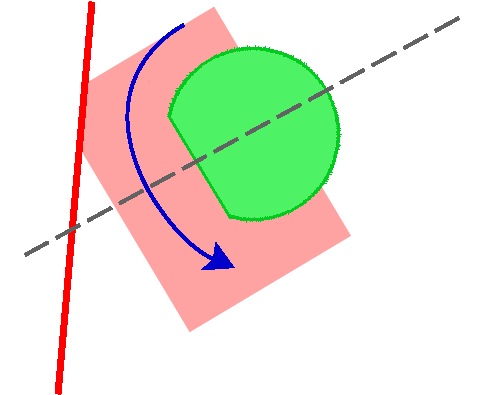
\includegraphics[width=0.5\textwidth]{driver-0.png}
  \caption{Description of the {\em driver-0} program function. The robot is
  drawn in green, the ``near field'' in light red, and the current
  straight-line path as a dashed gray line. The ``near field'' intersects the
  wall obstacle. Due to the bias in how the obstacle and the ``near field''
  intersect, a torque is generated that instructs the robot to scan for the
  next clear path in the counter-clockwise direction.}
  \label{fig:driver-0}
\end{figure}

\begin{enumerate}
  \item Obtain an up-to-date point cloud.
  \item Process the point cloud into a cost map and assign the average point
    height plus the variance in height of all points that fall in a particular
    2d grid cell as the cost for that cell.
  \item Observe the ``near field'' of the map for cells with a high cost where
    the ``near field'' is simply a region of interest near the robot.  Compute
    for each scanline of the ``near field'' a torque based on the lever from
    the robot center to the cell. Threshold all cells below a certain threshold
    to have zero torque.
  \item Check for a sudden drop in point cloud density. This may indicate an
    obstruction within $1$m of the robot.
  \item Update the driver state based on the near-field state and point cloud
    density. If there is no torque and high density, continue straight. When
    there is an obstacle to the left of the robot, a torque indicating that the
    robot should scan right will result. The opposite scan direction is emitted
    for an obstacle to the right. A low point cloud density will force the
    robot to enter a scanning mode.
  \item Send a velocity message to {\tt /cmd\_vel} based on the current robot
    state. For straight driving, use a constant linear velocity only. For a
    scan state, use a constant angular velocity only.
  \item Goto step $1$.
\end{enumerate}

\subsection{Observations}
The behavior of this simple program models loosely a particle under an elastic
collision with a wall. The robot will move in straight-line paths throughout
the environment, scanning for the next unobstructed direction in the most
efficient direction upon detection of a near collision.

When the robot encounters a wall, it is very sensitive to the size of the
``near field'' in terms of when the scanning state terminates and straight-line
motion resumes.  It would be best to encourage paths that drive parallel to
environment boundaries in order to explore the limits of the space. For this
reason, an enhancement to {\em driver-0} is to make the ``near field'' ROI a
trapezoid shape so that the robot will tend to exit a scan next to a wall
sooner and travel in a direction that is more parallel.

A very essential feedback mechanism that is not implemented in {\em driver-0}
is the iRobot Create bump sensor. For such a naive driving program, the bump
sensor can initiate a scan state and avoid behavior that causes the robot to
get stuck driving into an obstacle that it cannot see. Thin chair legs, thick
wires, or furniture with legs set on relatively thin bases can all become
obstructions that will be subtle in the cost map. In the absence of planning,
these features disappear due to the range limitations of the Kinect. Therefore,
the event of hitting them is often the only way to discern their presence.

The most severe limitation of this approach is that the Kinect provides no data
for depths less than $1$m, and so the forgetful nature of using only
instantaneous maps causes many common obstacles to disappear. Since the
intention of {\em driver-0} was to explore as much of the space as possible, it
often came too close to obstacles and then fell victim to the near-range
blindness of the Kinect. A more conservative threshold when defining a ``near
field'' would improve this behavior in the future with a corresponding loss in
``adventurous'' behavior since many smaller spaces will not be traversable
using a larger ``near field''.

\section{Visual odometry}
An instantaneous map alone cannot provide enough data to perform planning
functions with the robot since anything not immediately within the
field-of-view of a sensor is completely ignored. There are many algorithms that
can operate on a 2d grid to produce paths between two points in a map. Examples
include
\begin{enumerate}
  \item Brushfire
  \item Medial axis using distance operator
  \item Astar and variants
\end{enumerate}

All code relevant to visual odometry and mapping is contained in the files {\tt
demos/blr/feature-map.lsh} and {\tt demos/blr/prototype.lsh}. The function
{\tt xyz2global-feature-map-test} in {\tt prototype.lsh} implements the main
loop used to test visual odometry.

\subsection{Mapping}
A robust and coherent map of the environment is required to perform planning.
Each instantaneous viewpoint must be integrated into the global map using some
kind of matching. While the robot provides its own odometry, the inexpensive
IMU sensors and unreliable wheel speed measurements lead to odometry
measurements that have a substantial error. 

\begin{figure}
  \centering
  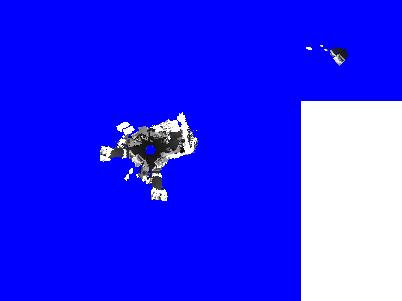
\includegraphics[width=0.5\textwidth]{lab_scans/lab_scan_odom_only_03.png}
  \caption{A full $360^{\circ}$ scan of the robotics lab on the 12th floor of
  NYU 719 Broadway. Error on the range of $90^{\circ}$ is common for a scan
  that uses only data from {\tt /robot\_pose\_ekf/odom} in order to register
  successive viewpoints into the global map.}
  \label{fig:lab_scan_odom_only}
\end{figure}

Figure~\ref{fig:lab_scan_odom_only} shows that a typical $360^{\circ}$ sweep of
a room with a smooth floor surface will result in a rotational error of nearly
$90^{\circ}$ despite the sensor fusion capabilities of {\tt
/robot\_pose\_ekf/odom}. This is not sufficient to do planning since even a
very small space cannot be mapped accurately.

\subsection{Feature correspondence}
Given two successive viewpoints $V_i$, $V_{i+1}$, and a mapping where for a
given interest point $m_i$ in $V_i$, the mapping gives the corresponding
location of the interest point in $V_{i+1}$, one can compute parameters that
describe a rigid transformation taking $V_i$ to $V_{i+1}$.

Therefore, the task in visual odometry is to find such correspondences using
features that can identify uniquely regions in one viewpoint and the same
region in the next viewpoint.

Many techniques exist for this problem including
\begin{itemize}
  \item SIFT/SURF, image space feature correspondence
  \item SLAM, probabilistic point cloud matching
  \item Kinect Fusion, voxel-based hardware accelerated mapping
\end{itemize}

Since the goal was to use the correspondence for planning, the more
sophisticated methods listed above were not used for this project since they
can have increasing data storage costs and implementation hurdles. Instead,
features extracted from the XYZRGB point cloud directly were used.

Features were collected at each cell of the 2d grid describing the map of
the environment, where each cell integrated data from all points whose $x$ and
$y$ coordinates fell within the axis-aligned bounding box of the cell grid. In
other words, cells took features from all points whose projection to the ground
plane fell within that cell's 2d coordinate bounds. Both depth and RGB features
were extracted to build up the local and global feature maps.

The first feature based on depth was simply a histogram whose $N$ bins each
describe a range of $z$ values. By counting the number of points at a given
cell that fall in each of the height ranges, a histogram is constructed that
approximates the distribution of heights at a given cell. A vertical wall would
correspond to a fairly uniformly distributed histogram whereas a table would
have samples only in the bin near the table surface.

In conjunction with the height histogram, the median RGB color for all points
falling within a particular height histogram bin was computed in order to
differentiate cell appearance. The justification for using the median is that
it is better suited to expressing a unique color without blending in samples
that are likely to be shared in common between cells such as a wall color or
other background data. Using a mean would tend to make cells look similar, even
when they have a dominant unique color.

Euclidean distance was used to score features as being unique and also as being
a match between the local and global maps. A threshold on the ratio of the
euclidean distance of the match to the length of the originating feature was
used rather than an absolute threshold since features in the space extracted
have no unit length.

\subsection{Experiments}
Using $15$ bins and a grid cell size of $10$cm provided optimal results. The
fact that the test environment was cluttered was ideal, and this approach would
fail very badly in a uniform environment. On average, scans using visual
odometry had error on the range of $30^{\circ}$ compared to $90^{\circ}$ for
those using odometry only. In general, error accumulates in a very non-linear
fashion. While there is error inherent to the discretization of the space
itself, the major cause of error is when the viewpoint passes over regions for
which the features lose their discriminative power. Either erroneous
correspondences will result, leading to a rapid jump in the map, or the map
will appear artificially similar and ``smear'' in place rather than update
properly in accordance with the robot motion.

Figure~\ref{fig:lab_scan_typical} shows a typical result for mapping with
visual odometry using the method outlined in this document.
Figure~\ref{fig:lab_scan_exceptional} shows that perseverance can be rewarded
with a coherent scan. However, for a proper visual odometry system we would
expect results like Figure~\ref{fig:lab_scan_exceptional} to be repeatable
rather than exceptional.

\begin{figure}
  \centering
  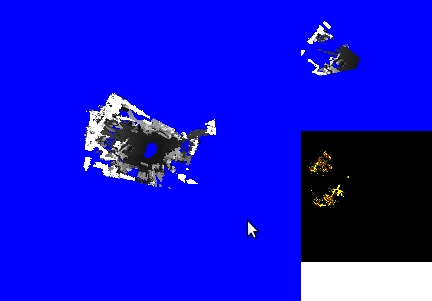
\includegraphics[width=0.5\textwidth]{lab_scans/lab_scan_03.png}
  \caption{A full $360^{\circ}$ scan of the robotics lab on the 12th floor of
  NYU 719 Broadway. Error on the range of $30^{\circ}$ is common for a scan
  that using both odometry data from {\tt /robot\_pose\_ekf/odom} as well as
  inter-frame visual odometry from feature correspondences.}
  \label{fig:lab_scan_typical}
\end{figure}

\begin{figure}
  \centering
  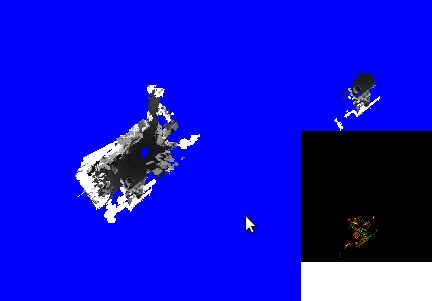
\includegraphics[width=0.5\textwidth]{lab_scans/lab_scan_06.png}
  \caption{A full $360^{\circ}$ scan of the robotics lab on the 12th floor of
  NYU 719 Broadway. An exceptional result was obtained using using both
  odometry data from {\tt /robot\_pose\_ekf/odom} as well as inter-frame visual
  odometry from feature correspondences.}
  \label{fig:lab_scan_exceptional}
\end{figure}

\subsection{Observations}
The biggest issue with the system implemented and the biggest question for such
systems in general is whether or not the features used possess sufficient
discriminative power to provide robust estimates of camera pose. In this case,
the pursuit of computational efficiency and compact representation were
favored, but at the expense of a feature that was robust enough to capture a
variety of environments.

Most of the variation in results was obtained by changing the grid size and
altering the permissiveness of the feature matching step. The grid size acts
similarly to an image pyramid by changing the scale of the features. This could
be implemented explicitly in order to try to improve the results. The best
results were obtained by computing two iterations on the same scale map.  The
first iteration would provide a larger search window to match the global map.
The output from the first iteration was then used to reprocess the local map
from the source point cloud before computing a second iteration using a
limited search window. A pyramid would replace the iterations on the same scale
map and allow features to emerge at different scales.

Another possible enhancement is to subtract the mode color of the current
local map in order to bias the search for colors that are unique. For indoor
environments, this would attempt to suppress the wall color, perhaps allowing a
signal for some other color in the cell to emerge instead.

Ultimately, it is very possible that the features selected in this method are
not unique enough to provide stable correspondences. In that case, using a
proven feature extraction algorithm like SIFT or SURF in the camera RGB image
would suffice, followed by storing the feature in its corresponding grid cell
in the map. Using such features would also be better suited to a different
data structure than the map since such features would be very sparse in
comparison to the dense map constructed for this project.

Still, a bare hallway that lacks edges would also fail when using SIFT. In this
case, plane fitting and odometry may be the only viable options.

%\subsection{Epilogue}
%In the previous section, the following enhancements to the visual odometry
%system are proposed:
%\begin{itemize}
%  \item Mode color suppression
%  \item Image pyramid
%\end{itemize}

\end{document}
